\chapter{Mathematical Induction}

\section{Recursion and Induction}

When we say that the natural numbers are the numbers $0$, $1$, $2$, $\ldots$, we really mean that the natural numbers are generated from $0$ and the \define{successor function} $S$ given by $n\mapsto n+1$.

As we saw in our exposition on the history of the concept of number, the definition of the natural numbers centers on precisely expressing the idea that all numbers are generated from $0$ and a successor function. Several ways of expressing this idea have been proposed through history: Dedekind's simply infinite sets, Peano's axioms, and the structural induction principle of type theory. We will follow the type-theoretic approach.

\begin{definition}
  The set $\mathbb{N}$ of natural numbers is a set equipped with an element $0$ and a successor function $S:\mathbb{N}\to\mathbb{N}$ given by $n\mapsto n+1$, satisfying the following principle of \define{structural induction}: For any family of sets $A_n$ indexed by the natural numbers equipped with
  \begin{enumerate}
  \item an element $a_0\in A_0$, and
  \item for each $n$, a function $h_n:A_n\to A_{n+1}$,
  \end{enumerate}
  there is a function $f$ taking a natural number $n$ as input and returning a value $f(n)$ in the set $A_n$, satisfying the following two equations:
  \begin{align*}
    f(0) & = a_0, \\
    f(n+1) & = h_n(f(n)).
  \end{align*}
\end{definition}

Thus, when defining a function by structural induction there are two subtasks: First, we have to specify the value of $f(0)$ by specifying an element of the set $A_0$, and second, we have to specify how each potential value of $f$ at $n$ can be used to obtain the value of $f$ at $n+1$. This second task is performed by defining a function $h_n$ from $A_n$ to $A_{n+1}$, so that if $f(n)$ is determined, then we can determine $f(n+1)$ by applying $h_n$ to $f(n)$.

The two equations that the function $f$ in the structural induction principle satisfies are called the \emph{computation rules}. By these computation rules we can present definitions by structural induction in the following shorthand form:
\begin{align*}
  f(0) & := a_0, \\
  f(n+1) & := h_n(f(n)).
\end{align*}

An important special case of structural induction, which will serve as our first example and by which we will define many further examples of recursive functions, is to \emph{iterate} any function $f$ on any set $X$. Here, we pick $A_n:= X$ for each $n$ (so it is not dependent on $n$), and we define $h_n:X\to X$ by $h:=f$ (again, not dependent on $n$). In the following definition we give the precise definition of the $n$\supth{} iteration of $f$.

\begin{definition}
  Consider a function $f:X\to X$. For each natural number $n$, we define the \define{$n$\supth{} iteration} $f^n$ of $f$ by
  \begin{align*}
    f^0(x) & := x, \\
    f^{n+1}(x) & := f(f^n(x)). 
  \end{align*}  
\end{definition}

In other words, the $0$\supth{} iteration of $f$ is the \define{identity function}, which leaves all elements untouched, and the $(n+1)$\supst{} iteration of $f$ is obtained by applying $f$ once more to the values of the $n$\supth{} iteration of $f$.

\begin{remark}\label{remark:alternative-iteration}
  Notice that we made a choice in the definition of the $(n+1)$\supst{} iteration of $f$. We could have defined it alternatively by $f^{n+1}(x):=f^n(f(x))$. In order to prove that the identity
  \begin{equation*}
    f^{n+1}(x)=f^n(f(x))
  \end{equation*}
  indeed holds we will need mathematical induction, which can be derived from structural induction.  
\end{remark}

\begin{definition}
  The principle of \define{mathematical induction} asserts that for any predicate $P(n)$ (that is, for any property of numbers depending on $n$), if
  \begin{enumerate}
  \item the proposition $P(0)$ holds, and
  \item for any $n$, if the proposition $P(n)$ holds then the proposition $P(n+1)$ holds,
  \end{enumerate}
  then $P(n)$ is true for all $n$.
\end{definition}

\begin{remark}
  Proofs by induction can thus be broken down into the following steps:
  \begin{enumerate}
  \item First identify the property $P(n)$ that you want to prove by induction. The goal of an induction proof is always to prove that $P(n)$ is true for all $n$.
  \item Next, prove the \emph{base case}. In other words, show that $P(0)$ is a true proposition. While this step is often trivial, it is a necessary and essential part of an induction proof.
  \item Finally, for the \emph{inductive step}, write down the exact \emph{induction hypothesis}, namely the property $P(n)$, and the exact goal of the inductive step, namely the property $P(n+1)$. Then use the induction hypothesis to prove that $P(n+1)$ then also holds.
  \end{enumerate}
  After these steps the proof that $P(n)$ holds is complete. Using induction we can prove, for example, that the identity $f^{n+1}(x)=f^n(f(x))$ holds for every $n$.  
\end{remark}

We are now in position to fully address \zcref{remark:alternative-iteration}.

\begin{proposition}\label{proposition:iterate-successor}
  Consider a function $f:X\to X$ on a set $X$, and let $n$ be a natural number. Then we have
  \begin{equation*}
    f^{n+1}(x) = f^n(f(x))
  \end{equation*}
  for all $x\in X$.
\end{proposition}

\begin{proof}
  The proof is by induction on $n$. In the base case, we must show that
  \begin{equation*}
    f^1(x) = f^0(f(x)).
  \end{equation*}
  By our definition of $f^n(x)$, we have that $f^1(x)=f(f^0(x))$, and we have $f^0(x)=x$, so that
  \begin{equation*}
    f^1(x)=f(f^0(x))=f(x).
  \end{equation*}
  Likewise, we have $f^0(f(x))=f(x)$. Therefore, it follows that both $f^1(x)=f(x)$ and $f^0(f(x))=f(x)$, which proves the base case.

  In the inductive step, we assume as our inductive hypothesis that the equality
  \begin{equation*}
    f^{n+1}(x)=f^n(f(x))
  \end{equation*}
  holds for every $x\in X$. Our goal is then to show that
  \begin{equation*}
    f^{n+2}(x)=f^{n+1}(f(x)).
  \end{equation*}
  Recall from the definition of iteration that $f^{n+2}(x)=f(f^{n+1}(x))$. Since we have assumed as our inductive hypothesis that the equality $f^{n+1}(x)=f^n(f(x))$ holds, we can continue our calculation as follows:
  \begin{equation*}
    f^{n+2}(x) = f(f^{n+1}(x)) = f(f^n(f(x))).
  \end{equation*}
  To finish the proof, we note that $f^{n+1}(y)=f(f^n(y))$. Choosing $y:=f(x)$, we obtain that $f^{n+1}(f(x))=f(f^n(f(x)))$. Thus we have shown the two equalities
  \begin{equation*}
    f^{n+2}(x) = f(f^n(f(x))) \qquad\text{and}\qquad f^{n+1}(f(x)) = f(f^n(f(x))),
  \end{equation*}
  so the inductive step is complete.
\end{proof}

\section{Addition of Natural Numbers}

Iterating functions is a basic operation that we can use to define many further operations. For example, addition is defined by iteratively adding $1$ to a number $m$. In other words, addition is defined by iterating the successor function. The $n$\supth{} iteration of the successor function is denoted by $S^n$.

\begin{definition}
  The \define{addition operation} ${+}:\mathbb{N}\to\mathbb{N}\to\mathbb{N}$ is a binary operation defined by iterating the successor function $S$:
  \begin{equation*}
    m+n := S^n(m).
  \end{equation*}
  In other words, $m+n$ is the $n$\supth{} successor of $m$.
\end{definition}

For example $2+3$ is defined as $S(S(S(2)))$, which is equal to $S(S(3))$, which is equal to $S(4)$, which is equal to $5$.

The operation $m,n\mapsto m+n$ satisfies the equalities
\begin{align*}
  m+0 & = m, \\
  m+(n+1) & = (m+n)+1
\end{align*}
by definition. However, these are the only equalities given to us via the computation rules of the structural induction principle. Other equalities, such as the equalities
\begin{align*}
  0+n & = n, \\
  (m+1)+n & = (m+n)+1
\end{align*}
are also true, but require a short proof.

\begin{proposition}\label{proposition:unit-law-addition-nat}
  For any two natural numbers $m$ and $n$ we have
  \begin{align*}
    0+n & = n, \\
    (m+1)+n & = (m+n)+1.
  \end{align*}
\end{proposition}

\begin{proof}
  The proof of both equalities is by induction on $n$. For the base case of the first equality, note that the equality $0+0=0$ holds by definition. For the inductive step, assume that $0+n=n$. Then we have
  \begin{equation*}
    0+(n+1)=(0+n)+1= n+1.
  \end{equation*}
  For the base case of the second equality, note that the equalities $(m+1)+0=m+1=(m+0)+1$ hold by definition. For the inductive step, assume that $(m+1)+n=(m+n)+1$. Then we have
  \begin{equation*}
    (m+1)+(n+1)=((m+1)+n)+1=((m+n)+1)+1=(m+(n+1))+1.\qedhere
  \end{equation*}
\end{proof}

\begin{proposition}\label{proposition:iterate-add}
  For any function $f:X\to X$, we have
  \begin{equation*}
    f^{m+n}(x)=f^m(f^n(x)).
  \end{equation*}
\end{proposition}

\begin{proof}
  The proof is by induction on $n$. In the base case, we have $m+0=m$ and $f^0(x)=x$. Together, these identities give:
  \begin{equation*}
    f^{m+0}(x)=f^m(x)=f^m(f^0(x)).
  \end{equation*}
  For the inductive step, assume that for every element $x\in X$ we have $f^{m+n}(x)=f^m(f^n(x))$. Our goal is to show that
  \begin{equation*}
    f^{m+(n+1)}(x)=f^m(f^{n+1}(x)).
  \end{equation*}
  Here, we use that the equalities $m+(n+1)=(m+n)+1$ and $f^{n+1}(x)=f(f^n(x))$ hold by definition, and that the equality $f^m(f(x))=f(f^m(x))$ holds by \zcref{proposition:iterate-successor}. Together, these identities give:
  \begin{align*}
    f^{m+(n+1)}(x)=f^{(m+n)+1}(x) & =f(f^{m+n}(x))=f(f^m(f^n(x))) \\
                                  & =f^m(f(f^n(x)))=f^m(f^{n+1}(x)).\qedhere
  \end{align*}
\end{proof}

\begin{corollary}
  Addition of natural numbers is \define{associative}: For any three natural numbers $l$, $m$, and $n$ we have
  \begin{equation*}
    (l+m)+n = l+(m+n).
  \end{equation*}
\end{corollary}

\begin{proof}
  By definition, we have $(l+m)+n=S^n(S^m(l))$ and $l+(m+n)=S^{m+n}(l)$. Combining these identities with \zcref{proposition:iterate-add}, we obtain
  \begin{equation*}
    (l+m)+n=S^n(S^m(l))=S^{m+n}(l)=l+(m+n).\qedhere
  \end{equation*}
\end{proof}

\begin{proposition}
  Addition of natural numbers is \define{commutative}: For any two natural numbers $m$ and $n$, we have
  \begin{equation*}
    m+n=n+m.
  \end{equation*}
\end{proposition}

\begin{proof}
  The proof is by induction on $n$. In the base case, we use \zcref{proposition:unit-law-addition-nat}
  \begin{equation*}
    m+0=m=0+m.
  \end{equation*}
  For the inductive step, assume that $m+n=n+m$. Then we use \zcref{proposition:unit-law-addition-nat} again to obtain:
  \begin{align*}
    m+(n+1) & = (m+n)+1 \\
            & = (n+m)+1 \\
            & = (n+1)+m.
  \end{align*}
  This completes the induction step.
\end{proof}

Some further useful identifications of addition, which follow from the associativity and commutativity laws, are:
\begin{align*}
  (l+m)+n & = (l+n)+m, \\
  l+(m+n) & = m+(l+n), \\
  (k+l)+(m+n) & = (k+m)+(l+n).
\end{align*}
The last identification is called the \define{interchange law} for addition. The first one follows from the second, and the second and third are proven by a short calculation:
\begin{align*}
  l+(m+n) & = (l+m)+n & (k+l)+(m+n) & = k+(l+(m+n)) \\
          & = (m+l)+n & & = k + (m + (l+n)) \\
          & = m+(l+n), & & = (k+m)+(l+n).
\end{align*}

\section{Arithmetic of Natural Numbers}

\begin{definition}
  The \define{multiplication function} $m,n\mapsto mn$ on the natural numbers is defined recursively by
  \begin{align*}
    m0 & := 0, \\
    m(n+1) & := mn + m.
  \end{align*}
\end{definition}

\begin{proposition}
  Multiplication of natural numbers satisfies the following laws:
  \begin{align*}
    0n & = 0, & m0 & = 0, \\
    (m+1)n & = mn+n, & m(n+1) & = mn+m, \\
    1m & = m, & m1 & = m, \\
    l(m+n) & = lm+ln, & (l+m)n & = ln+mn, \\
    (lm)n & = l(mn), & mn & = nm.
  \end{align*}
\end{proposition}

\begin{proof}
  We prove that $0n=0$ by induction on $n$. In the base case, we have the equality $00=0$. For the inductive step, assume that $0n=0$. Then $0(n+1)=0n+0=0n=0$, completing the proof of the first identity. The identity $m0=0$ holds by definition.

  The proof that $(m+1)n=mn+n$ is again by induction on $n$. In the base case, we have the equalities $(m+1)0=0=m0=m0+0$. For the inductive step, assume that $(m+1)n=mn+n$. Then we have
  \begin{align*}
    (m+1)(n+1)
    & = (m+1)n+(m+1) \\
    & = (mn+n)+(m+1) \\
    & = (mn+m)+(n+1) \\
    & = m(n+1)+(n+1).
  \end{align*}
  The identity $m(n+1)=mn+m$ holds by definition.

  Next, we prove first that $mn=nm$, by induction on $n$. In the base case, we have the equalities $m0=0=0m$. For the inductive step, assume that $mn=nm$. Then we have that
  \begin{equation*}
    m(n+1)=mn+m=nm+m=(n+1)m.
  \end{equation*}

  Now we prove that $l(m+n)=lm+ln$. We prove it by induction on $n$. In the base case, we have that $l(m+0)=lm=lm+0= lm+l0$. For the inductive step, assume that $l(m+n)=lm+ln$. Then we have that
  \begin{equation*}
    l(m+(n+1))=l((m+n)+1)=l(m+n)+l=(lm+ln)+l=lm+(ln+l)=lm+l(n+1).
  \end{equation*}
  The identification $(l+m)n=ln+mn$ follows from the previous identification, using the fact that $mn=nm$.

  Finally, the proof that $(lm)n=l(mn)$ is by induction on $n$. In the base case, we have the equalities $(lm)0=0=l0=l(m0)$. For the inductive step, assume that $(lm)n=l(mn)$. Then we have that
  \begin{equation*}
    (lm)(n+1)= (lm)n+lm=l(mn)+lm=l(mn+m)=l(m(n+1)).
  \end{equation*}
  This completes the inductive step.
\end{proof}

\section{Relations on the Natural Numbers}

Among Peano's axioms are the axioms stating that $0$ is not a successor and that the successor function is injective. Recall that a function $f:X\to Y$ is called \define{injective} if the following implication holds:
\begin{equation*}
  f(x)=f(y)\quad\Rightarrow\quad x=y.
\end{equation*}
As the reader may have duly noted, we have neither postulated that $0$ is not a successor and that the successor function is injective. Our goal is to prove them.

\begin{example}
  We define the binary operation $E:\mathbb{N}\to(\mathbb{N}\to\mathcal{P}(\symbf{1}))$ by defining
  \begin{align*}
    E(0,0) & := \top, & E(0,n+1) & := \bot, \\
    E(m+1,0) & := \bot, & E(m+1,n+1) & := E(m,n).
  \end{align*}
  We can prove by induction that the proposition $E(m,n)$ is true if and only if $m=n$. For the forward direction, we have to show that if $E(m,n)$ is true, then $m=n$. This is proven by double induction: the proposition $E(0,0)$ is true by definition, and indeed we have $0=0$; the propositions $E(0,n+1)$ and $E(m+1,0)$ are both false by definition; and if $E(m+1,n+1)$ is true, then $m=n$ by the inductive hypothesis, which implies that $m+1=n+1$.

  For the converse, we have to show that if $m=n$, then $E(m,n)$ is true. In other words, we need to show that $E(n,n)$ is true for each natural number $n$. Indeed, the proposition $E(0,0)$ is true by definition, and the proposition $E(n+1,n+1)=E(n,n)$ is true by the inductive hypothesis.
\end{example}

This simple example allows us to prove the two properties Peano postulated as axioms.

\begin{theorem}
  The natural number $0$ is not a successor.
\end{theorem}

\begin{proof}
  Suppose that $0=n+1$ for some natural number $n$. This equality implies that
  \begin{equation*}
    E(0,0)=E(0,n+1).
  \end{equation*}
  In other words, we have that $\symbf{1}=\varnothing$. Thus we conclude that $\top=\bot$, which is absurd.
\end{proof}

\begin{theorem}
  The successor function is injective.
\end{theorem}

\begin{proof}
  Suppose that $m+1=n+1$. Then the proposition $E(m+1,n+1)$ is true, and consequently we find that the proposition $E(m,n)$ is true. This shows that $m=n$.
\end{proof}

\begin{example}
  We end with the inductive definitions of the inequality relations $\leq$ and $<$. These are defined by first defining binary operations
  \begin{equation*}
    R_{\leq},R_{<}:\mathbb{N}\to(\mathbb{N}\to\mathcal{P}(\symbf{1})).
  \end{equation*}
  Both of these operations are defined recursively:
  \begin{align*}
    R_{\leq}(0,0) & := \symbf{1}, & R_{\leq}(0,n+1) & := \symbf{1}, \\
    R_{\leq}(m+1,0) & := \varnothing & R_{\leq}(m+1,n+1) & := R_{\leq}(m,n). \\
    \intertext{and}
    R_{<}(0,0) & := \varnothing, & R_{<}(0,n+1) & := \symbf{1}, \\
    R_{<}(m+1,0) & := \varnothing & R_{<}(m+1,n+1) & := R_{<}(m,n).
  \end{align*}
  Now we define $m\leq n$ to hold if and only if $R_{\leq}(m,n)$ contains an element, and we define $m<n$ to hold if and only if $R_{<}(m,n)$ contains an element.
\end{example}

\begin{remark}
  We have an obligation to mention why Peano postulated these two properties as axioms. Peano was working in a logical framework that was much weaker than set theory. In particular, the system in which he formulated the axioms for the natural numbers contained no powersets. The \define{powerset} $\mathcal{P}(A)$ of a set $A$ is a set whose elements are subsets $U\subseteq A$.
  
  For example, let $\symbf{1}:=\{\ast\}$ be the singleton set containing only the element $\ast$. Then the powerset $\mathcal{P}(\symbf{1})$ contains the empty subset $\varnothing\subseteq \symbf{1}$ and the full subset $\symbf{1}\subseteq\symbf{1}$. More generally, for every proposition $P$, we have the subset
  \begin{equation*}
    \{\ast\mid P\}\subseteq \{\ast\},
  \end{equation*}
  which contains the element $\ast$ only when the proposition $P$ holds. For example, when $P:=\bot$ is the false proposition, then the subset $\{\ast\mid\bot\}$ is empty, and when $P:=\top$ is the true proposition, then the subset $\{\ast\mid\top\}$ contains the element $\ast$.
  
  Our reason for considering the powerset $\mathcal{P}(\symbf{1})$ is that we can define relations on the natural numbers by recursively defining maps
  \begin{equation*}
    \mathbb{N}\to (\mathbb{N}\to \mathcal{P}(\symbf{1})).
  \end{equation*}
\end{remark}

\section{Finite Sums and Products}

\begin{definition}
  The \define{finite summation operation} $\sum$ is defined by specifying a finite subset $I\subseteq \mathbb{N}$ and a family of natural numbers $a_i$ where $i$ ranges over the elements of $I$. We will write
  \begin{equation*}
    \sum_{i\in I}a_i
  \end{equation*}
  for the sum over all the natural numbers $a_i$, with $i$ ranging over $I$. This sum is defined by recursion over the number of elements in $I$. If $I$ has no elements (that is, $I$ is empty), then we define
  \begin{equation*}
    \sum_{i\in I}a_i := 0.
  \end{equation*}
  If $I$ has at least one element $i_0$, then we write $J:=I\setminus\{i_0\}$, allowing us to define
  \begin{equation*}
    \sum_{i\in I}a_i := a_{i_0}+\sum_{i\in J}a_j.
  \end{equation*}
\end{definition}

\begin{theorem}
  For any natural number $n$ we have
  \begin{equation*}
    0 + \cdots + n = \frac{n(n+1)}{2}.
  \end{equation*}
\end{theorem}

\begin{proof}
  Let $S_n:=0+\cdots+n$, and let $P(n)$ be the property that $S_n=\frac{n(n+1)}{2}$. We will prove that $P(n)$ is true for all $n$ by induction. In the base case, we have to show that $P(0)$ holds, that is, that the identity
  \begin{equation*}
    0=\frac{0\cdot 1}{2}
  \end{equation*}
  is true. This is indeed true, because the numerator in the fraction on the right-hand side is $0$.

  For the induction step, let $n$ be a natural number and assume as our inductive hypothesis that $P(n)$ is true. Our goal is now to prove $P(n+1)$, that is, that the identity
  \begin{equation*}
    S_{n+1}=\frac{(n+1)(n+2)}{2}.
  \end{equation*}
  Note that $S_{n+1}=S_n+(n+1)$. By the inductive hypothesis we have that $S_n=\frac{n(n+1)}{2}$, which we may now use to rewrite
  \begin{equation*}
    S_n + (n+1) = \frac{n(n+1)}{2} + (n+1).
  \end{equation*}
  Observe that $(n+1)=\frac{2(n+1)}{2}$. Therefore we can make the following computation:
  \begin{equation*}
    \frac{n(n+1)}{2} + (n+1) = \frac{n(n+1)}{2}+\frac{2(n+1)}{2} = \frac{n(n+1)+2(n+1)}{2}=\frac{(n+2)(n+1)}{2}.
  \end{equation*}
  Since $(n+2)(n+1)=(n+1)(n+2)$ it follows that $S_{n+1}=\frac{(n+1)(n+2)}{2}$ as desired.
\end{proof}

We illustrate induction with another example, the \define{formula for the geometric series}.

\begin{theorem}\label{theorem:formula-geometric-series}
  For any real number $x$ not equal to $1$, the identity
  \begin{equation*}
    \sum_{k=0}^{n-1}x^k = \frac{x^n-1}{x-1}.
  \end{equation*}
\end{theorem}

\begin{proof}
  The proof is by induction on $n$. In the case $n=0$ the sum
  \begin{equation*}
    \sum_{k=0}^{-1}x^k
  \end{equation*}
  is an empty sum, because it sums over all elements $0\leq k \leq -1$ of which there are none. In empty sums, nothing is being added, so they are always $0$. On the right hand side, we also see that
  \begin{equation*}
    \frac{x^0-1}{x-1}=\frac{1-1}{x-1}=0,
  \end{equation*}
  and hence the base case holds.

  For the inductive step, assume that $\sum_{k=0}^{n-1}x^k=\frac{x^n-1}{x-1}$. Our goal is to show that
  \begin{equation*}
    \sum_{k=0}^{n}x^k=\frac{x^{n+1}-1}{x-1}.
  \end{equation*}
  Note that $\sum_{k=0}^{n}x^k=(\sum_{k=0}^{n-1}x^k)+x^n$. By applying the induction hypothesis we therefore find that
  \begin{equation*}
    \sum_{k=0}^{n}x^k=\frac{x^n-1}{x-1}+x^n.
  \end{equation*}
  Note that $x^n=\frac{(x-1)x^n}{x-1}$. Therefore we can bring the two summands under one fraction as follows:
  \begin{equation*}
    \frac{x^n-1}{x-1}+x^n=\frac{x^n-1}{x-1}+\frac{(x-1)x^n}{x-1}=\frac{x^n-1+x^{n+1}-x^n}{x-1}=\frac{x^{n+1}-1}{x-1}.
  \end{equation*}
  This completes the inductive step, and therefore the proof.
\end{proof}

\section{Hemachandra's Counting Problem}
\label{section:hemachandra}

\begin{figure}[t]
  \centering
  \tagpdfparaOff
  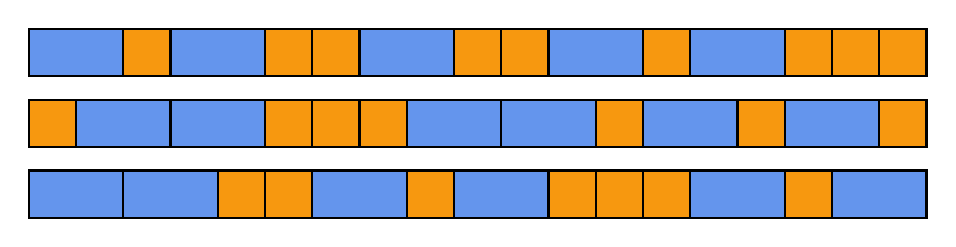
\begin{tikzpicture}[scale=0.6]
    % --- first tiling (a) at y=0 ---
    \begin{scope}[shift={(0,0)}]
      % tiles: 2,1,2,1,1,2,1,1,2,1,2,1,1,1
      \foreach \x/\len in {
        0/2, 2/1, 3/2, 5/1, 6/1, 7/2, 9/1,
        10/1, 11/2, 13/1, 14/2, 16/1, 17/1, 18/1
      }{
        \ifnum\len=1
          \fill[YellowOrange] (\x,0) rectangle ++(1,1);
        \else
          \fill[CornflowerBlue] (\x,0) rectangle ++(2,1);
        \fi
        \draw[thick] (\x,0) rectangle ++(\len,1);
      }
    \end{scope}
    
    % --- second tiling (b) at y=-1.5 ---
    \begin{scope}[shift={(0,-1.5)}]
      % tiles: 1,2,2,1,1,1,2,2,1,2,1,2,1
      \foreach \x/\len in {
        0/1, 1/2, 3/2, 5/1, 6/1, 7/1, 8/2,
        10/2, 12/1, 13/2, 15/1, 16/2, 18/1
      }{
        \ifnum\len=1
          \fill[YellowOrange] (\x,0) rectangle ++(1,1);
        \else
          \fill[CornflowerBlue] (\x,0) rectangle ++(2,1);
        \fi
        \draw[thick] (\x,0) rectangle ++(\len,1);
      }
    \end{scope}
    
    % --- third tiling (c) at y=-3 ---
    \begin{scope}[shift={(0,-3)}]
      % tiles: 2,2,1,1,2,1,2,1,1,1,2,1,2
      \foreach \x/\len in {
        0/2, 2/2, 4/1, 5/1, 6/2, 8/1, 9/2,
        11/1, 12/1, 13/1, 14/2, 16/1, 17/2
      }{
        \ifnum\len=1
          \fill[YellowOrange] (\x,0) rectangle ++(1,1);
        \else
          \fill[CornflowerBlue] (\x,0) rectangle ++(2,1);
        \fi
        \draw[thick] (\x,0) rectangle ++(\len,1);
      }
    \end{scope}
  \end{tikzpicture}
  \tagpdfparaOn
  \caption[Some Hemachandra tilings of a 1-by-19 grid]{\label{figure:fibonacci-tilings}Three example tilings of a 1-by-19 grid using monominoes (1-by-1 tiles) and dominoes (1-by-2 tiles).}
\end{figure}

In the 12\supth{} century, the Indian scholars Gopāla and Hemachandra studied the number of rhythmic patterns formed by combining short and long syllables in Sanskrit prosody. Hemachandra, around the year 1150, found a systematic way of counting the number of rhythmic patterns that can occur for any number of beats.

In order to rediscover Hemachandra's method, it might be helpful to think of the patterns of short and long syllables in terms of tilings one can make on a 1-by-$n$ grid using monominoes (1-by-1 tiles) and dominoes (1-by-2 tiles). We have displayed some arbitrary examples of such tilings in \zcref{figure:fibonacci-tilings}. The question is thus: How many such patterns are there?

In order to count them, let $H_n$ be the number of such tilings. One way of finding the number $H_n$, which works when a specific $n$ is given, is to simply list all the tilings of a 1-by-$n$ grid. Doing so for small values of $n$ is a great way to get a feeling for the problem. In \zcref{figure:complete-fifth-fibonacci-tiling} we have listed all the possible tilings of the 1-by-5 grid.
\begin{figure}[t]
  \centering
  \tagpdfparaOff
  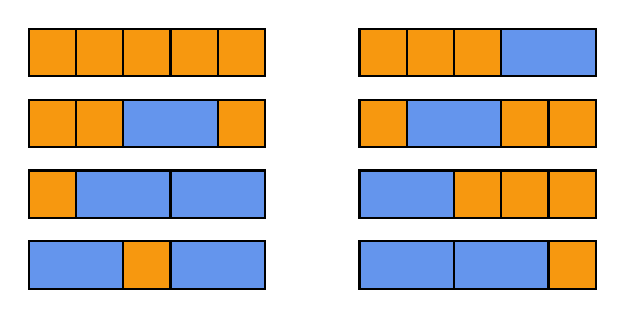
\begin{tikzpicture}[scale=0.6]
    % Colours
    \definecolor{mono}{RGB}{255,165,0}   % monomino
    \definecolor{domi}{RGB}{100,149,237} % domino
    
    % Helper: draw one tiling given a shift and a list of x/length pairs
    \newcommand{\drawtiling}[3]{%
      \begin{scope}[shift={(#1,#2)}]
        \draw[step=1cm,gray!40] (0,0) grid (5,1);
        \foreach \x/\len in {#3} {
          \ifnum\len=1
            \fill[YellowOrange] (\x,0) rectangle ++(1,1);
            \draw[thick] (\x,0) rectangle ++(1,1);
          \else
            \fill[CornflowerBlue] (\x,0) rectangle ++(2,1);
            \draw[thick] (\x,0) rectangle ++(2,1);
          \fi
        }
      \end{scope}%
    }
    
    % Now place the 8 tilings in two columns
    % Each list is x/length so that the tiles exactly fill 0..5
    \drawtiling{0}{   0}{0/1,1/1,2/1,3/1,4/1}   % 1 1 1 1 1
    \drawtiling{7}{   0}{0/1,1/1,2/1,3/2}       % 1 1 1 2
    \drawtiling{0}{ -1.5}{0/1,1/1,2/2,4/1}      % 1 1 2 1
    \drawtiling{7}{ -1.5}{0/1,1/2,3/1,4/1}      % 1 2 1 1
    \drawtiling{7}{ -3  }{0/2,2/1,3/1,4/1}      % 2 1 1 1
    \drawtiling{0}{ -3  }{0/1,1/2,3/2}          % 1 2 2
    \drawtiling{0}{ -4.5}{0/2,2/1,3/2}          % 2 1 2
    \drawtiling{7}{ -4.5}{0/2,2/2,4/1}          % 2 2 1
    
  \end{tikzpicture}
  \tagpdfparaOn
  \caption[Hemachandra tilings of a 1-by-5 grid]{\label{figure:complete-fifth-fibonacci-tiling}A list of all the possible tilings of a 1-by-5 grid using monominoes and dominoes.}
\end{figure}

For the first few numbers it is easy to determine the value of $H_n$. For example, the number $H_1$ is just $1$, since the only way of tiling a 1-by-1 grid using monominoes and dominoes is to use a single monomino. Likewise, the number $H_2$ is $2$, since we can either use two monominoes or one domino as a tiling of a 1-by-2 grid. However, listing all such tilings gets elaborate for larger $n$ quite quickly, and furthermore doing so by hand is quite error-prone. The problem is therefore to find a clever way of counting all possible patterns for all $n$.

Notice that the last tile is either a monomino or a domino, so there are two cases to consider. The number of tilings ending in a monomino is exactly the number $H_{n-1}$, and the number of tilings ending in a domino is exactly the number $H_{n-2}$. This can be seen in \zcref{figure:complete-fifth-fibonacci-tiling}, where we listed all the tilings of the 1-by-5 grid. There are five tilings ending in a monomino, corresponding to each of the five different tilings of the 1-by-4 grid. Similarly, there are three tilings ending in a domino, corresponding to the three different tilings of the 1-by-3 grid. Thus, the total number of tilings of a 1-by-$n$ grid is the sum of these two numbers:
\begin{equation*}
  H_n = H_{n-1} + H_{n-2}.
\end{equation*}
This recursive rule is very famous: It is the rule that generates the \emph{Fibonacci numbers}.

\begin{definition}
  The sequence $F_n$ of \define{Fibonacci numbers} is defined by
  \begin{equation*}
    F_0:= 0,\qquad F_1:= 1,\qquad\text{and}\qquad F_{n+2}=F_{n+1}+F_{n}.
  \end{equation*}
\end{definition}

Since the numbers $H_n$ start with $H_1=1$ and $H_2=2$, we find that
\begin{equation*}
  H_n = F_{n+1}.
\end{equation*}
Hemachandra applied this recurrence to list the initial values of the sequence $H_n$:  $1$, $2$, $3$, $5$, $8$, $13$, $21$. His results appear in his treatise on metrics, the \emph{Chandonuśāsana} \cite{hemachandra1961}, composed several decades before Fibonacci's \emph{Liber Abaci} (1202). Nevertheless, in most of the world this sequence of numbers is called the Fibonacci numbers, even though it might be more appropriate to call them the Hemachandra--Fibonacci numbers.

The tiling interpretation of the Fibonacci numbers also appears in \cite{brigham1996}. The delightful book \emph{Proofs That Really Count: The Art of Combinatorial Proof} by Arthur Benjamin and Jennifer Quinn uses the tiling interpretation of the Fibonacci numbers to derive many Fibonacci identities combinatorially, and it contains many further examples of beautiful counting constructions \cite{benjamin2003}.

\clearpage%

\exercises

\begin{starter}
  \exercise \label{exercise:sum-of-odd-numbers}Prove that the sum of the first $n$ odd numbers is a perfect square. That is, prove that
  \begin{equation*}
    \sum_{k=0}^{n-1} 2k+1 = n^2.
  \end{equation*}
  Note: This summation formula is the starting point from which Fibonacci derived much of his work in his book  \emph{Liber Quadratorum (The Book of Squares)} \cite{fibonacci1987}.
  \exercise
  \begin{subexenum}
  \item Prove that
    \begin{equation*}
      \sum_{k=0}^nF_k = F_{n+2}-1.
    \end{equation*}
  \item Prove that
    \begin{equation*}
      \sum_{k=0}^{n-1}F_{2k+1}=F_{2n}.
    \end{equation*}
  \item Prove that
    \begin{equation*}
      \sum_{k=0}^{n}F_{2k}=F_{2n+1}-1.
    \end{equation*}
  \end{subexenum}  
  \exercise Just as in Hemachandra's counting problem, suppose we have a metre of $n$ beats composed of long ($2$ beats) and short syllables ($1$ beat). This time, the short syllables are distinguished between strong or soft beats. Write down the recursive formula for the number of rhythmic patterns of $n$ beats, and use it to determine the correct values for $1\leq n\leq 10$.
  \exercise \label{exercise:hemachandra-variant}Consider strips subdivided into $n$ blocks, in which some blocks are colored blue, so that no two colored blocks are adjacent. For example, the following is a valid coloring of the strip with $10$ blocks:
  \begin{center}
    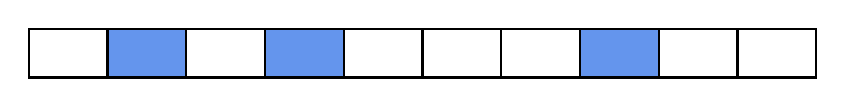
\begin{tikzpicture}
      \def\L{10}
      \def\H{.62}
      \def\n{10}
      \pgfmathsetmacro{\step}{\L/\n}
      
      \foreach \k in {1,3,7} {
        \fill[CornflowerBlue] (\k*\step,0) rectangle ++(\step,\H);
      }
      
      \draw[thick] (0,0) rectangle (\L,\H);
      
      \foreach \k in {1,...,9} {
        \draw[thick] (\k*\step,0) -- (\k*\step,\H);
      }
    \end{tikzpicture}
  \end{center}
  Let $C_n$ be the number of such colorings. Find $C_1$ and $C_2$, and express $C_{n+2}$ in terms of $C_{n+1}$ and $C_{n}$.
\end{starter}

\begin{routine}
  \exercise \label{exercise:difference-of-powers}
  Prove the \define{formula for the difference of $n$\supth{} powers}
  \begin{equation*}
    x^n-y^n=(x-y)\sum_{k=0}^{n-1}x^ky^{n-1-k}.
  \end{equation*}
  Note that this formula generalizes the \define{formula for the difference of squares}
  \begin{equation*}
    x^2-y^2 = (x-y)(x+y)
  \end{equation*}
  as well as the \define{formula for the geometric series}
  \begin{equation*}
    x^n-1=(x-1)\sum_{k=0}^{n-1} x^k.
  \end{equation*}
  \exercise \label{exercise:identities-triangular-numbers}Write $T_n$ for the $n$\supth{} triangular number.
  \begin{subexenum}
  \item For $0\leq m<n$, show that
    \begin{equation*}
      T_n-T_m=\frac{(n-m)(n+m+1)}{2}.
    \end{equation*}
  \item For any two natural numbers $m$ and $n$, show that
    \begin{equation*}
      T_{m+n}=T_{m}+T_n+mn.
    \end{equation*}
  \item Show that
    \begin{equation*}
      T_{2n}=4T_n-n.
    \end{equation*}
  \item Show that
    \begin{equation*}
      8T_n+1=(2n+1)^2.
    \end{equation*}
  \end{subexenum}
  \exercise Write $T_n$ for the $n$\supth{} triangular number, and define the \define{$n$\supth{} tetrahedral number} $S_n$ by
  \begin{equation*}
    S_n:=\sum_{k=0}^nT_k.
  \end{equation*}
  \begin{subexenum}
  \item Give a geometric interpretation of these numbers justifying their name.
  \item Prove that
    \begin{equation*}
      S_n = \frac{n(n+1)(n+2)}{6}.
    \end{equation*}
  \item Prove that
    \begin{equation*}
      S_{m+n}=S_m+S_n+\frac{mn(m+n+2)}{2}.
    \end{equation*}
  \end{subexenum}
  \exercise
  \begin{subexenum}
  \item
    Prove the \define{formula for the square pyramidal numbers}
    \begin{equation*}
      \sum_{k=0}^n k^2 = \frac{n(n+1)(2n+1)}{6}.
    \end{equation*}
    Can you explain why the numbers of the form $\sum_{k=0}^n k^2$ are called square pyramidal numbers?
  \item Prove that
    \begin{equation*}
      \sum_{k=0}^{n-1}(2k+1)^2 = \frac{n(4n^2-1)}{3}.
    \end{equation*}
  \end{subexenum}
  \exercise
  \begin{subexenum}
  \item Prove \define{Nicomachus's Theorem}
    \begin{equation*}
      \sum_{k=0}^n k^3 = \left(\sum_{k=0}^{n}k\right)^2.
    \end{equation*}
  \item Prove that
    \begin{equation*}
      \sum_{k=0}^{n-1}(2k+1)^3=n^2(2n^2-1).
    \end{equation*}
  \end{subexenum}
  \exercise Prove that
  \begin{equation*}
    \sum_{k=0}^n k(k+1)(k+2) = \frac{n(n+1)(n+2)(n+3)}{4}.
  \end{equation*}
  \exercise Prove that
  \begin{equation*}
    \sum_{k=0}^n F_k^2 = F_nF_{n+1}.
  \end{equation*}
\end{routine}

\begin{foundational}
  \exercise Consider a function $f:X \to X$. Show that for any $x\in X$ the following equality holds:
  \begin{equation*}
    f^n(f^m(x))=f^m(f^n(x)).
  \end{equation*}
  \exercise Consider a function $f:X \to X$. Show that for any $x\in X$, the following equality holds:
  \begin{equation*}
    f^{mn}(x)=(f^m)^n(x).
  \end{equation*}
  \exercise For any natural number $m$, consider the function
  \begin{equation*}
    I_m : (X\to X) \to (X\to X)
  \end{equation*}
  defined by $I_m(f):= f^m$. We can iterate this function too! Prove that for any function $f:X\to X$ and any $x\in X$, the following equality holds:
  \begin{equation*}
    f^{m^n}(x) = (I_m)^n(f)(x).
  \end{equation*}
  \exercise Show that the function $x\mapsto x+n$ is \define{injective}, meaning that the following implication holds:
  \begin{equation*}
    x+n=y+n\qquad\Rightarrow\qquad x=y.
  \end{equation*}
\end{foundational}

\begin{challenge}
  \exercise
  \begin{subexenum}
  \item Prove \define{Cassini's identity}:
    \begin{equation*}
      F_{n+1}^2-F_nF_{n+2}=(-1)^n.
    \end{equation*}
  \item Prove the following generalization of Cassini's identity:
    \begin{equation*}
      F_{n+k}^2 - F_{n}F_{n+2k} = (-1)^n F_k^2.
    \end{equation*}
  \end{subexenum}
  \exercise Consider two nonzero natural numbers $a$ and $b$ satisfying $a(a+b) < b^2$. Prove that the strict inequality
  \begin{equation*}
    F_n<\left(\frac{b}{a}\right)^n
  \end{equation*}
  holds for all $n$. Use Cassini's identity to give some examples of natural numbers $a$ and $b$ that satisfy this inequality.
  \exercise Show that
  \begin{equation*}
    F_{2n+1}^2+F_{2n+3}^2+1 = 3F_{2n+1}F_{2n+3}.
  \end{equation*}
  \exercise \label{exercise:arithmetic-progression-fibonacci}Define
  \begin{align*}
    a_n & := F_{n}F_{n+1}- (-1)^n, \\
    b_n & := F_{n}^2 + F_{n+1}^2, \\
    c_n & := 3F_{n}F_{n+1}+(-1)^{n}.
  \end{align*}
  Show that $(a_n^2,b_n^2,c_n^2)$ is an \define{arithmetic progression of squares}; that is, show that
  \begin{equation*}
    b_n^2-a_n^2=c_n^2-b_n^2.
  \end{equation*}
  \exercise A \define{$3$-term arithmetic progression} $(a,b,c)$ is a triple of numbers $a\leq b\leq c$ with common increment, so that $b-a=c-b$. Show that every 3-term arithmetic progression of distinct positive Fibonacci numbers is of the form
  \begin{equation*}
    (F_n,F_{n+2},F_{n+3}).
  \end{equation*}
  Conclude that there are no 4-term arithmetic progressions of distinct positive Fibonacci numbers.
  \exercise Let $A_n$ be the number of maps $f:\{1,\ldots, n\}\to\{1,2,3\}$ satisfying the condition that
  \begin{equation*}
    \min(f(i),f(j))\leq |i-j|
  \end{equation*}
  for any two distinct elements $1\leq i,j\leq n$.
  \begin{subexenum}
  \item Compute the numbers $A_1$, $A_2$, $A_3$, and $A_4$.
  \item Find a recursive expression for $A_{n+4}$.
  % Answer: A_{n+4} = A_{n+3} + A_{n+2} + A_{n+1} + A_{n}.
  \end{subexenum}
  \exercise Consider the numbers $s_n$ given by
  \begin{equation*}
    s_0:=0,\qquad s_1:=1,\qquad\text{and}\qquad s_{n+2}=34s_{n+1}-s_n+2.
  \end{equation*}
  The first few numbers in this sequence are $0,1,36,1225,41616, 1413721, 48024900,\ldots$.
  \begin{subexenum}
  \item Show that $s_n$ is a square number for each $n$.
  \item Show that $s_n$ is a triangular number for each $n$.
  \end{subexenum}
\end{challenge}

%%% Local Variables:
%%% mode: latex
%%% TeX-master: "elementary-number-theory"
%%% TeX-engine: luatex
%%% End:

